\documentclass{article}
\usepackage{indentfirst}
\usepackage[utf8]{inputenc}
\usepackage[T1]{fontenc}
\usepackage[brazilian]{babel}
\usepackage{lmodern}
\usepackage{graphicx}
\usepackage{float}
\usepackage[]{subfigure}
\usepackage{afterpage}
\usepackage{amsmath}
\usepackage{textcomp,gensymb}
\usepackage{nameref}
\usepackage{accents}
\usepackage{listings}
\usepackage{color,soul}
\usepackage[margin=1in]{geometry}
\usepackage{steinmetz}
\usepackage{xfrac}

\PassOptionsToPackage{hyphens}{url}\usepackage{hyperref}
\hypersetup{
    breaklinks = true,
}
\urlstyle{same}
\newcommand{\ubar}[1]{\underaccent{\bar}{#1}}
%\renewcommand\thesection{\arabic{section}$^a$}
\renewcommand\thesection{\arabic{section}.}
\renewcommand\thesubsection{\arabic{section}.\alph{subsection}}
\definecolor{dkgreen}{rgb}{0,0.6,0}
\definecolor{gray}{rgb}{0.5,0.5,0.5}
\definecolor{mauve}{rgb}{0.58,0,0.82}
\lstset{
    frame=tb,
    language=Matlab,
    aboveskip=3mm,
    belowskip=3mm,
    showstringspaces=false,
    basicstyle={\small\ttfamily},
    numbers=none,
    numberstyle=\tiny\color{gray},
    keywordstyle=\color{blue},
    commentstyle=\color{dkgreen},
    stringstyle=\color{mauve},
    breaklines=true,
    breakatwhitespace=true,
    tabsize=4
}

\title{Simulação 5 - Controle Digital}
\author{Arthur de Matos Beggs - 12/0111098}
\date{2021}

\begin{document}
% capa
\begin{titlepage}
    \begin{center}
        \centering
        
\includegraphics[width=.7\linewidth]{images/logo_unb.png}\\[0.5cm]
        {\large \textbf{Universidade de Brasília}}\\[0.2cm]
        {\large \textbf{Departamento de Engenharia Elétrica}}\\[0.2cm]
        {\large \textbf{Controle Digital}}\\[4.8cm]
        {\bf \huge {Exercício de Simulação 5}}\\[0.2cm]
        {\bf \large {}}
    \end{center}

    \vspace{5cm}
    \hspace{2cm} {\noindent \bf \large {Aluno:}}\\
    \vspace{0.8cm}
    \hspace{2.35cm} {\large Arthur de Matos Beggs --------------------------------- 12/0111098}\\[1cm]

    \begin{center}
        {\large Brasília}\\
        {\large 2$^{\ubar{\circ}}$/2020}
    \end{center}

\end{titlepage}

\clearpage % Quebra de página

\setcounter{page}{2}

    \section*{\normalsize{\normalfont Considere que a planta do sistema de
    controle a tempo discreto mostrado na Figura~\ref{fig:diagram} tem função
    de transferência}}

    \[ G(s) = \frac{10}{s(s+2)} \]

    \section*{\normalsize{\normalfont O período de amostragem é $T = 0.1\,s$.}}

    \begin{figure}[H]
       \centering
            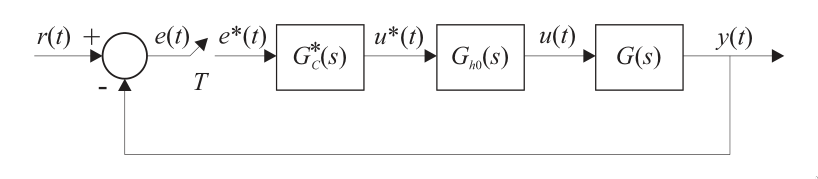
\includegraphics[width=1\linewidth]{images/diagrama.png}
            \caption{Diagrama do sistema.}
            \label{fig:diagram}
    \end{figure}

    \section{\normalsize{\normalfont Projete o controlador $G_c(z)$ de modo que
    o sistema em malha fechada tenha resposta $y[k]$ ao degrau com erro $e[k]$
    nulo para todo $k$ maior que um número finito de instantes de amostragem.
    O controlador $G_c(z)$ deve cancelar o zero da planta discretizada $G(z)$
    que fica dentro do CRU.}}

        {Discretizando a planta $G(s)$ com o \textit{ZOH} $G_{h0}(s)$,}

        \[ G(z) = \mathcal{Z}\left\{ G_{h0}(s)G(s)\right\}
                = (1-z^-1)\mathcal{Z}\left\{ \frac{10}{s^2(s+2)}\right\} \]

        {Pelo Matlab,}
        \begin{lstlisting}
T = 0.1;

s = tf('s');
z = tf('z', T);

G_s = zpk([], [0 -2], [10])
G_z = c2d(G_s, T, 'zoh')
        \end{lstlisting}

        \[ G(z) = \frac{0.046827(z+0.9355)}{(z-1)(z-0.8187)} \]

        {Para um sistema com resposta \textit{deadbeat},}

        \[ M(z) = \frac{Y(z)}{R(z)};\; G_c(z) = \frac{1}{G(z)}\frac{M(z)}{1-M(z)} \]

        {Onde}
        \[ M(z) = \prod_{i=1}^I (1-z_i z^{-1}) (M_{k} z^{-k} + M_{k+1} z^{-k-1} + \cdots) \]
        \[ 1 - M(z) = \prod_{j=1}^{J} (1-p_j z^{-1})(1-z^{-1})^p (1 + a_1 z^{-1} + a_2 z^{-2} + \cdots) \]
        {sendo $z_i,\; i = 1,\, 2,\, ...\,I$ os zeros da planta que não devem
            ser cancelados e $p_j,\; j = 1,\, 2,\, ...\,J$ os polos da planta
            que não devem ser cancelados.}

        \[ n = n_p[G(z)] - n_z[G(z)] = 2 - 1 = 1 \]
        \[ k = n_p[M(z)] - n_z[M(z)] \]

        {Para a resposta a tempo mínimo, $k = n = 1$.}
        {Considerando a entrada degrau $R(z) = \frac{z}{z-1}$,}

        \[ p = \mathrm{max}\left\{ n_p[R(z)] \mathrm{\,em\,} z=1,\,
                n_p[G(z)] \mathrm{\,em\,} z=1 \right\}
             = \mathrm{max}\left\{ 1, \,1 \right\}
             = 1 \]

        {Como o controlador deve cancelar o zero da planta,}
        \[ M(z) = (M_1 z^{-1} + M_2 z^{-2}) \]
        \[ 1 - M(z) = (1-z^{-1})^1 (1+ a_1 z^{-1}) \]
        \[ 1 - (M_1 z^{-1} + M_2 z^{-2}) = (1-z^{-1})^1 (1+ a_1 z^{-1})
            = 1-(1-a_1)z^{-1} - a_1 z^{-2} \]

        \[\begin{cases}
            M_1 = 1 - a_1\\
            M_2 = a_1
        \end{cases}\]

        {Escolhendo $a_1 = -1$, temos que $M_1 = 2$ e $M_2 = -1$.}
        \[ M(z) = (2z^{-1} - z^{-2}) = \frac{2(z-0.5)}{z^2} \]
        \[ 1 - M(z) = \frac{(z-1)^2}{z^2} \]

        {Assim,}
        \[ G_c(z) = \frac{1}{G(z)}\frac{M(z)}{1-M(z)}
                  = \frac{(z-1)(z-0.8187)}{0.046827(z+0.9355)}
                    \frac{2(z-0.5)}{z^2} \frac{z^2}{(z-1)^2}
                  = \frac{42.7104(z-0.5)(z-0.8187)}{(z-1)(z+0.9355)} \]


    \section{\normalsize{\normalfont Simule o sistema em malha fechada com o
    controlador projetado no item anterior conforme o diagrama da
    Figura~\ref{fig:diagram} para entrada degrau unitário. Faça os gráficos da
    saída $y(t)$ em tempo contínuo da planta $G(s)$, do sinal de erro $e[k]$
    que entra no controlador a tempo discreto $G_c(z)$ e do sinal de controle
    $u(t)$ que sai do segurador de ordem zero $G_{h0}(z)$.}}

        {Declarando o controlador $G_c(z)$ encontrado no \textit{workspace} do
        Matlab, o sistema da Figura~\ref{fig:q2_simulink} pode ser simulado.}
        \begin{lstlisting}
[Z_g, P_g, K_g] = zpkdata(G_z, 'v')
Gc1_z = zpk([0.5 P_g(2)], [1 Z_g(1)], [2/K_g], T)
        \end{lstlisting}

        \begin{figure}[H]
           \centering
                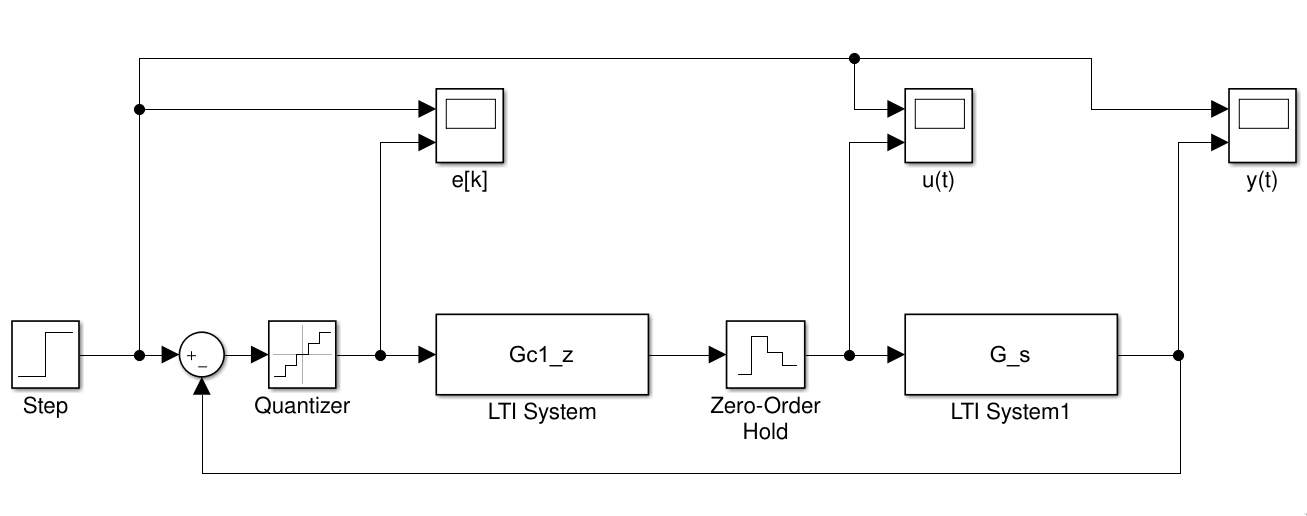
\includegraphics[width=.7\linewidth]{images/q2_simulink.png}
                \caption{Sistema simulado.}
                \label{fig:q2_simulink}
        \end{figure}

        {O sinal de saída $y(t)$ é mostrado na Figura~\ref{fig:q2_simulink_y}.
        Aparentemente o sinal chega no valor de referência em dois instantes de
        tempo e permanece no valor de referência. Porém, a
        Figura~\ref{fig:q2_simulink_y_zoom} com \textit{zoom} mostra que existem
        pequenas oscilações no sinal entre os momentos onde o sinal é amostrado.}

        \begin{figure}[H]
           \centering
                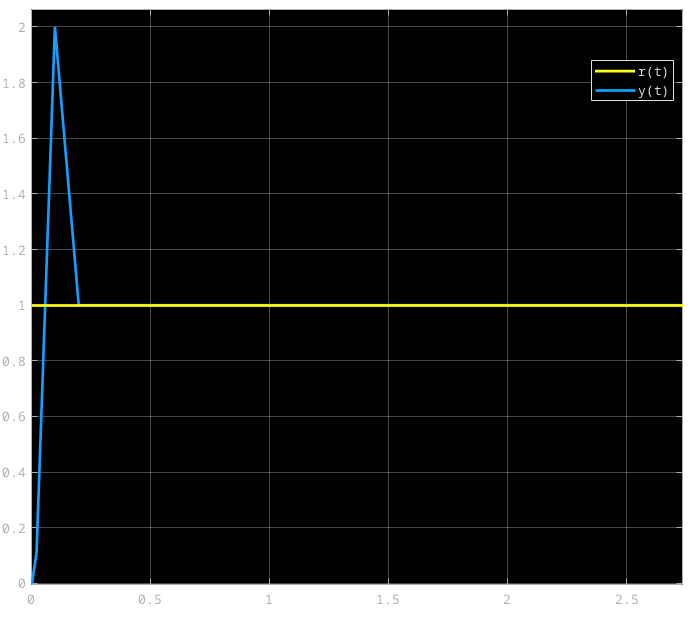
\includegraphics[width=.6\linewidth]{images/q2_y_t.png}
                \caption{Gráfico da resposta y(t).}
                \label{fig:q2_simulink_y}
        \end{figure}

        \begin{figure}[H]
           \centering
                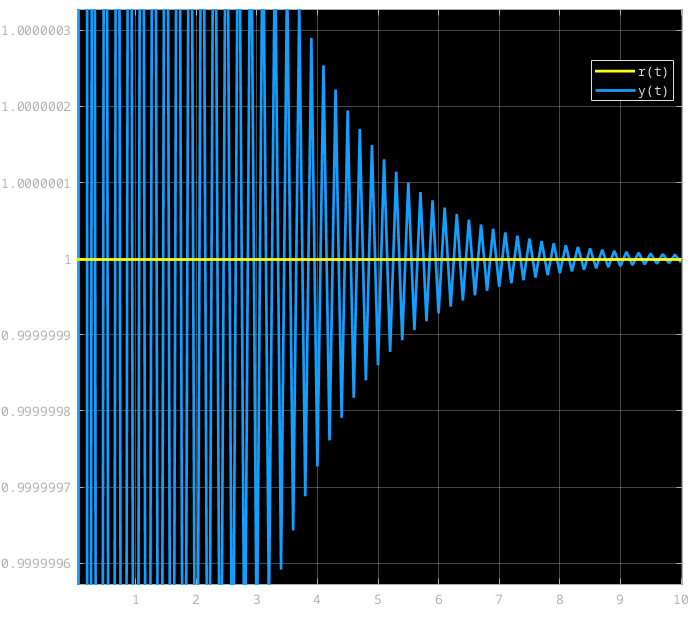
\includegraphics[width=.6\linewidth]{images/q2_y_t_zoom.png}
                \caption{Gráfico da resposta y(t) ampliado.}
                \label{fig:q2_simulink_y_zoom}
        \end{figure}

        {A Figura~\ref{fig:q2_simulink_e} mostra o sinal de erro $e[k] = 0$ em
        dois instantes de tempo.}

        \begin{figure}[H]
           \centering
                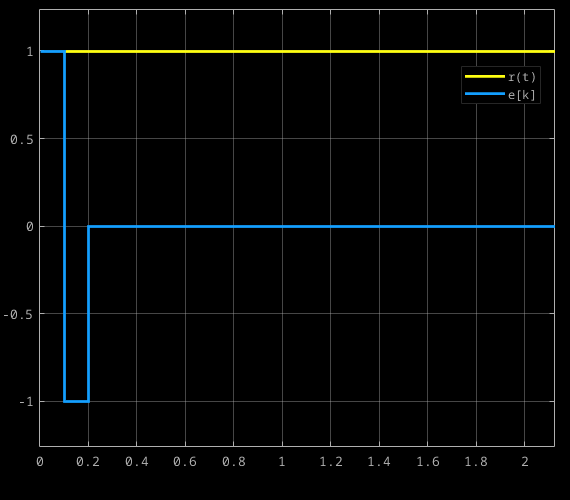
\includegraphics[width=.6\linewidth]{images/q2_e_k.png}
                \caption{Gráfico do sinal e[k].}
                \label{fig:q2_simulink_e}
        \end{figure}

        {A Figura~\ref{fig:q2_simulink_u} mostra o sinal de controle $u(t)$.}

        \begin{figure}[H]
           \centering
                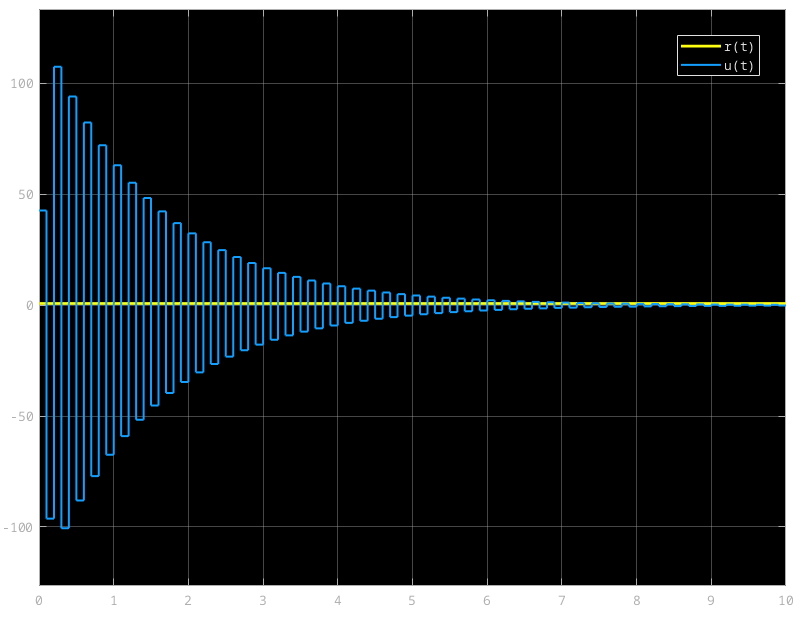
\includegraphics[width=.6\linewidth]{images/q2_u_t.png}
                \caption{Gráfico do sinal u(t).}
                \label{fig:q2_simulink_u}
        \end{figure}


    \section{\normalsize{\normalfont Projete o controlador $G_c(z)$ de modo que
    o sistema em malha fechada tenha resposta $y(t)$ ao degrau com erro $e(t)$
    nulo para todo $t$ maior que um número finito de instantes de amostragem.
    O controlador $G_c(z)$ não deve cancelar o zero da planta discretizada
    $G(z)$ que fica dentro do CRU.}}

        {Discretizando a planta $G(s)$ com o \textit{ZOH} $G_{h0}(s)$,}

        \[ G(z) = \mathcal{Z}\left\{ G_{h0}(s)G(s)\right\}
                = (1-z^-1)\mathcal{Z}\left\{ \frac{10}{s^2(s+2)}\right\} \]

        {Pelo Matlab,}
        \begin{lstlisting}
T = 0.1;

s = tf('s');
z = tf('z', T);

G_s = zpk([], [0 -2], [10])
G_z = c2d(G_s, T, 'zoh')
        \end{lstlisting}

        \[ G(z) = \frac{0.046827(z+0.9355)}{(z-1)(z-0.8187)} \]

        {Para um sistema com resposta \textit{deadbeat},}

        \[ M(z) = \frac{Y(z)}{R(z)};\; G_c(z) = \frac{1}{G(z)}\frac{M(z)}{1-M(z)} \]

        {Onde}
        \[ M(z) = \prod_{i=1}^I (1-z_i z^{-1}) (M_{k} z^{-k} + M_{k+1} z^{-k-1} + \cdots) \]
        \[ 1 - M(z) = \prod_{j=1}^{J} (1-p_j z^{-1})(1-z^{-1})^p (1 + a_1 z^{-1} + a_2 z^{-2} + \cdots) \]
        {sendo $z_i,\; i = 1,\, 2,\, ...\,I$ os zeros da planta que não devem
            ser cancelados e $p_j,\; j = 1,\, 2,\, ...\,J$ os polos da planta
            que não devem ser cancelados.}

        \[ n = n_p[G(z)] - n_z[G(z)] = 2 - 1 = 1 \]
        \[ k = n_p[M(z)] - n_z[M(z)] \]

        {Para a resposta a tempo mínimo, $k = n = 1$.}
        {Considerando a entrada degrau $R(z) = \frac{z}{z-1}$,}

        \[ p = \mathrm{max}\left\{ n_p[R(z)] \mathrm{\,em\,} z=1,\,
                n_p[G(z)] \mathrm{\,em\,} z=1 \right\}
             = \mathrm{max}\left\{ 1, \,1 \right\}
             = 1 \]

        {Como o controlador não deve cancelar o zero da planta,}
        \[ M(z) = (1 + 0.9355z^{-1}) (M_1 z^{-1}) \]
        \[ 1 - M(z) = (1-z^{-1})^1 (1+ a_1 z^{-1}) \]
        \[ 1 - ( (1 + 0.9355z^{-1}) (M_1 z^{-1}) ) = (1-z^{-1})^1 (1+ a_1 z^{-1})
            = 1-(1-a_1)z^{-1} - a_1 z^{-2} \]

        \[\begin{cases}
            M_1 = 1 - a_1 & \implies M_1 = \frac{1}{1.9355} = 0.5167\\
            a_1 = 0.9355M_1 & \implies a_1 = \frac{0.9355}{1.9355} = 0.4833
        \end{cases}\]

        \[ M(z) = (1 + 0.9355z^{-1}) (0.5167 z^{-1})
                = \frac{0.5167(z + 0.9355)}{z^2} \]
        \[ 1 - M(z) = (1-z^{-1})^1 (1+ 0.4833 z^{-1})
                = \frac{(z-1)(z+0.4833)}{z^2} \]

        {Assim,}
        \[ G_c(z) = \frac{1}{G(z)}\frac{M(z)}{1-M(z)}
                  = \frac{(z-1)(z-0.8187)}{0.046827(z+0.9355)}
                    \frac{0.5167(z + 0.9355)}{z^2} \frac{z^2}{(z-1)(z+0.4833)}
                  = \frac{11.033(z-0.8187)}{(z+0.4833)} \]


    \section{\normalsize{\normalfont Simule o sistema em malha fechada com o
    controlador projetado no item anterior conforme o diagrama da
    Figura~\ref{fig:diagram} para entrada degrau unitário. Faça os gráficos da
    saída $y(t)$ em tempo contínuo da planta $G(s)$, do sinal de erro $e[k]$
    que entra no controlador a tempo discreto $G_c(z)$ e do sinal de controle
    $u(t)$ que sai do segurador de ordem zero $G_{h0}(z)$.}}

        {Declarando o controlador $G_c(z)$ encontrado no \textit{workspace} do
        Matlab, o sistema da Figura~\ref{fig:simulink_4} pode ser simulado.}
        \begin{lstlisting}
[Z_g, P_g, K_g] = zpkdata(G_z, 'v')
a1 = -Z_g(1)/(1-Z_g(1))
M1 = 1/(1-Z_g(1))
Gc2_z = zpk([P_g(2)], [-a1], [M1/K_g], T)
        \end{lstlisting}

        \begin{figure}[H]
           \centering
                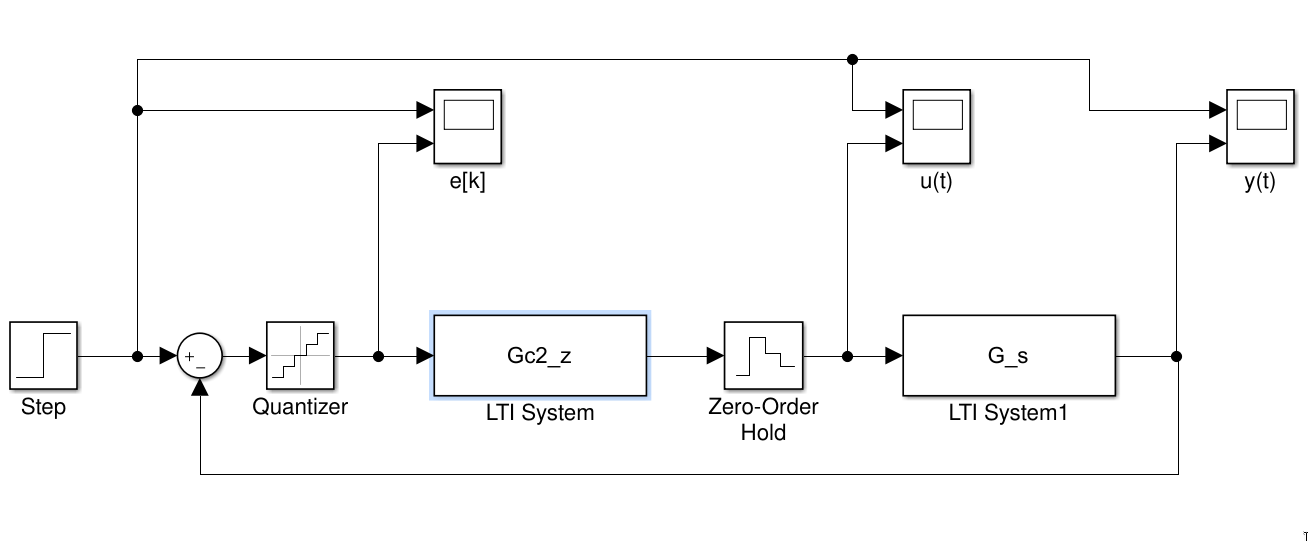
\includegraphics[width=.6\linewidth]{images/q4_simulink.png}
                \caption{Sistema simulado.}
                \label{fig:simulink_4}
        \end{figure}

        {O sinal de saída $y(t)$ é mostrado na Figura~\ref{fig:q4_simulink_y}.
        O sinal chega próximo ao valor de referência em dois instantes de
        amostragem.}

        \begin{figure}[H]
           \centering
                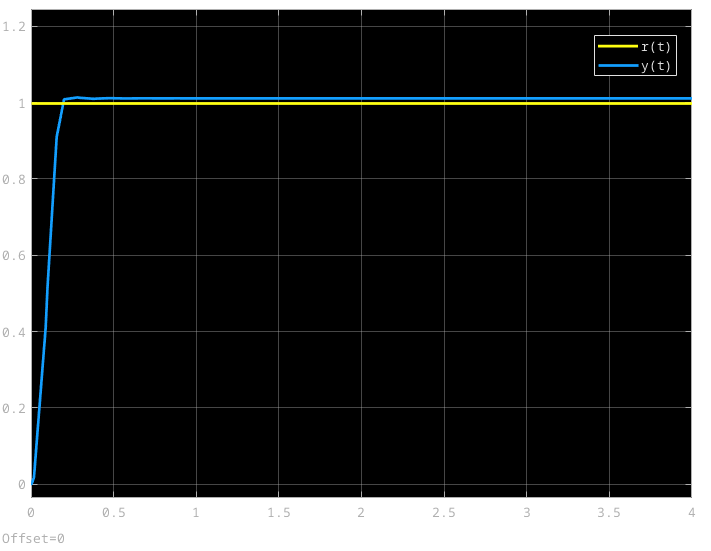
\includegraphics[width=.5\linewidth]{images/q4_y_t.png}
                \caption{Gráfico da resposta y(t).}
                \label{fig:q4_simulink_y}
        \end{figure}

        {O erro pode ser proveniente de problemas na simulação ou na
        resposta em tempo contínuo. A Figura~\ref{fig:q4_step} mostra a resposta
        da planta discretizada a uma entrada degrau unitário com erro nulo
        obtida por}
        \begin{lstlisting}
step(feedback(G_z*Gc2_z, 1))
grid on
        \end{lstlisting}

        \begin{figure}[H]
           \centering
                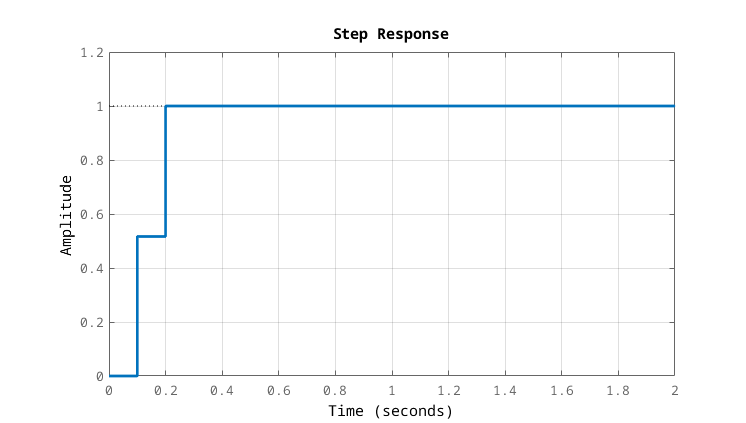
\includegraphics[width=.7\linewidth]{images/q4_step.png}
                \caption{Gráfico da resposta y(t) obtida com a planta discretizada.}
                \label{fig:q4_step}
        \end{figure}

        {A Figura~\ref{fig:q4_simulink_e} mostra o sinal de erro $e[k] = 0$ em
        dois instantes de tempo.}

        \begin{figure}[H]
           \centering
                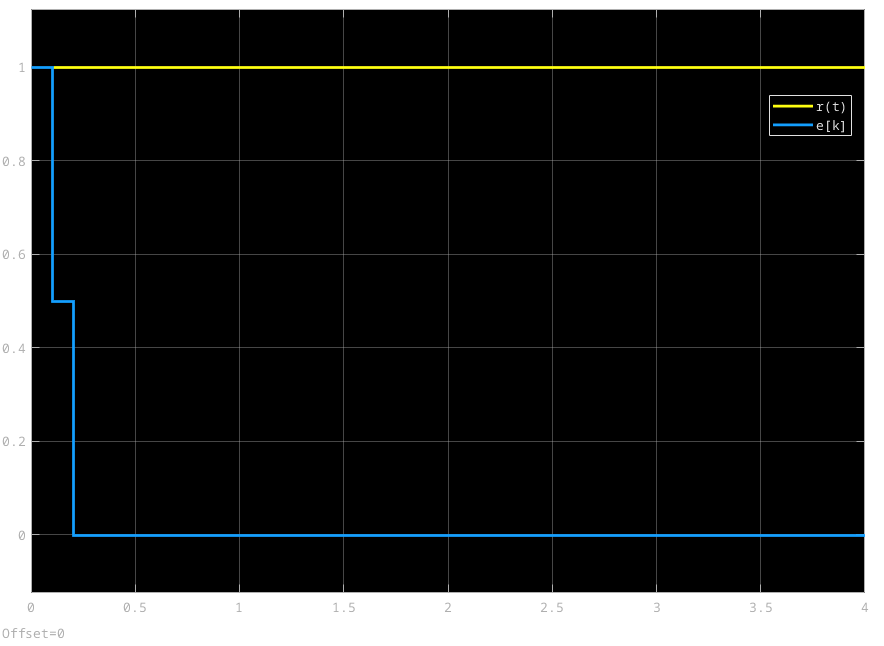
\includegraphics[width=.6\linewidth]{images/q4_e_k.png}
                \caption{Gráfico do sinal e[k].}
                \label{fig:q4_simulink_e}
        \end{figure}

        {A Figura~\ref{fig:q4_simulink_u} mostra o sinal de controle $u(t)$.}

        \begin{figure}[H]
           \centering
                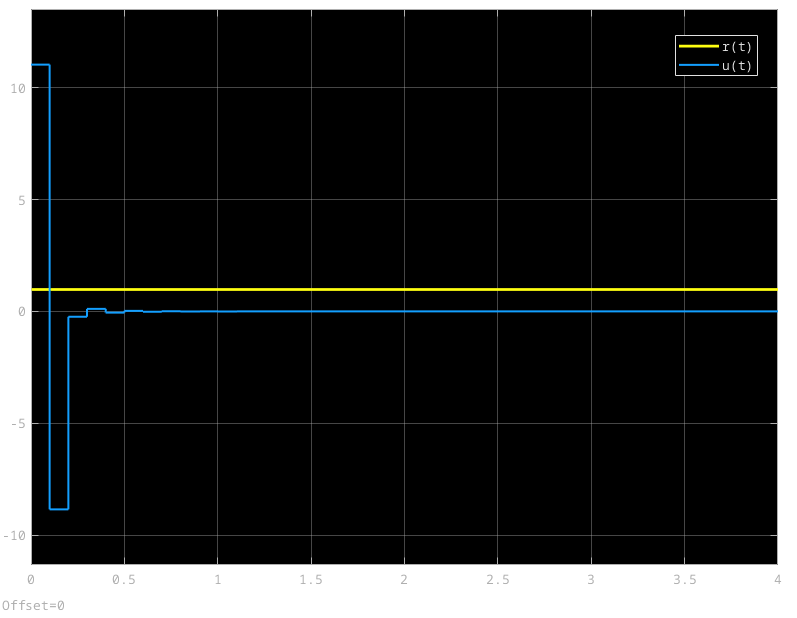
\includegraphics[width=.6\linewidth]{images/q4_u_t.png}
                \caption{Gráfico do sinal u(t).}
                \label{fig:q4_simulink_u}
        \end{figure}


\end{document}

